% =====================================================================
% sections/heterogeneity.tex — shared (long + short)
% =====================================================================

\section{Heterogeneity}
\label{sec:heterogeneity}

The pooled estimates of Section~\ref{sec:results} mask substantial
heterogeneity across subgroups. Three dimensions are reported.

\paragraph{By sex.}
The headline pattern from Table~\ref{tab:main_results_by_sex} is that
the health-index gain is concentrated among girls. This replicates the
central qualitative finding of the predecessor DEPII analysis. The
female health-index estimate is several times larger than the male
estimate; both are imprecisely estimated, but the gap is substantively
meaningful and consistent with two channels suggested by the prior
literature. \textcite{frankenberg2005} document that midwives' antenatal
and postnatal services disproportionately reach female infants in
Indonesia. \textcite{makowiecka2008} observe that the program's
nutrition-counseling component, in particular, has stronger uptake
among mothers of girls, plausibly because the marginal returns to
nutritional supplementation are larger for girls in settings where
boys are favored at the household level.

\paragraph{By mother's education.}
Table~\ref{tab:het_medu} splits the sample by whether the mother's
years of schooling are above or below the median in the analysis
sample (six years). The depression-index point estimate is larger
among children of less-educated mothers, consistent with the program
being a substitute for, rather than a complement to, maternal education
in the production of child mental health. The health-index split is
flatter and the cognition-index split shows no clear pattern.

\begin{table}[!htbp]
\centering
\caption{Heterogeneity by mother's years of schooling.}
\label{tab:het_medu}
% Auto-generated by code/R/12_heterogeneity_finalize.R
\begin{tabular}{lcc}
\toprule
Outcome & Low-edu mother & High-edu mother \\
\midrule
Health index & \makecell{-0.013\\(0.084)} & \makecell{-0.454\\(0.186)} \\
Cognition index & \makecell{-0.035\\(0.073)} & \makecell{-0.148\\(0.160)} \\
Depression index & \makecell{-0.030\\(0.090)} & \makecell{0.158\\(0.200)} \\
Socioemotional index & \makecell{-0.073\\(0.084)} & \makecell{0.015\\(0.215)} \\
\bottomrule
\end{tabular}

\begin{minipage}{0.8\textwidth}
\footnotesize
\emph{Notes.} TWFE estimates with community-of-birth and birth-year
fixed effects, estimated separately on the sub-medianeducation
($\leq 6$ years) and above-medianeducation subsamples. Standard
errors clustered at the community-of-birth level.
\end{minipage}
\end{table}

\paragraph{By exposure window.}
Table~\ref{tab:het_age} reports separate coefficients for being in
utero, aged 0--3, aged 4--6, or aged 7+ at the time of the village
midwife's arrival, with the never-treated and pre-program cohorts as
the omitted reference. The pattern is consistent with a critical-period
interpretation: the health-index point estimates are largest in the
in-utero and 0--3 windows and shrink toward zero for older children.
The cognition and Big-Five indices show little structure across
windows. The depression-index estimate is positive in every window but
imprecise.

\begin{table}[!htbp]
\centering
\caption{Heterogeneity by age window at rollout.}
\label{tab:het_age}
% Auto-generated by code/R/12_heterogeneity_finalize.R
\begin{tabular}{lcccc}
\toprule
Outcome & In utero & Age 0--3 & Age 4--6 & Age 7+ \\
\midrule
health\_index & \makecell{-0.020\\(0.067)} & \makecell{-0.075\\(0.054)} & \makecell{-0.005\\(0.047)} & \makecell{---} \\
cognition\_index & \makecell{-0.030\\(0.068)} & \makecell{0.011\\(0.048)} & \makecell{-0.023\\(0.036)} & \makecell{---} \\
depression\_index & \makecell{-0.039\\(0.065)} & \makecell{-0.023\\(0.051)} & \makecell{-0.046\\(0.041)} & \makecell{---} \\
bigfive\_index & \makecell{0.010\\(0.066)} & \makecell{0.000\\(0.053)} & \makecell{-0.011\\(0.044)} & \makecell{---} \\
\bottomrule
\end{tabular}

\begin{minipage}{0.85\textwidth}
\footnotesize
\emph{Notes.} TWFE estimates with community-of-birth and birth-year
fixed effects. Each column is a separate dummy in the same regression;
the omitted reference is the union of never-treated and pre-program
(treated after age 7) cohorts. Standard errors clustered at the
community-of-birth level.
\end{minipage}
\end{table}

The forest plot in Figure~\ref{fig:forest} summarizes the four
outcomes across all five subgroups: full sample, male, female,
low-education mother, high-education mother.

\begin{figure}[!htbp]
\centering
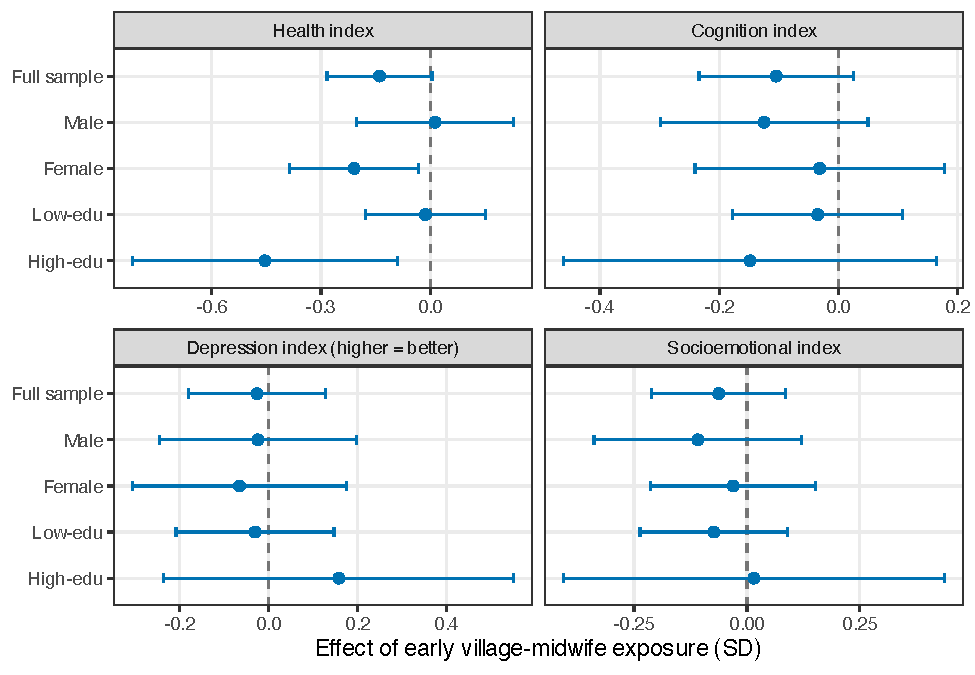
\includegraphics[width=0.92\textwidth]{figures/heterogeneity_forest.pdf}
\caption{Heterogeneity forest plot: TWFE point estimates and 95\%
confidence intervals across subgroups.}
\label{fig:forest}
\end{figure}

\paragraph{Why might cognition fail to respond?}
The absence of a measurable cognitive effect is consistent with the
distinction between fluid and crystallized cognitive abilities
discussed by \textcite{tuckerdrob2022}: fluid abilities, measured by
the IRT number-series score \texttt{w\_abil}, decline with age
beginning in early adulthood, while crystallized abilities continue to
accumulate. The mean age of the analysis sample at wave~5 is~22, by
which point any cognitive premium from early-life nutrition or care
may have begun to attenuate. A complementary reading is that the
cognitive scales available in IFLS are noisy proxies for the
underlying construct.
